\documentclass[a4paper,12pt]{article}
\usepackage{a4wide}
\usepackage{amsmath,amsthm}
\usepackage[utf8]{inputenc}
\usepackage[english]{babel}
\usepackage{enumerate}
\usepackage{tikz}
    \usetikzlibrary{arrows,automata,positioning}

\theoremstyle{definition}
    \newtheorem{problem}{Problem}

\begin{document}

\begin{center}
    \large{NTIN071 A\&G: Homework assignment}    
\end{center}


{\it  Each problem is worth 5 points, totaling 20 points. The solution must be entirely your own work. Describe all steps in your solution, the objects you construct, and proofs in sufficient detail and using the formalism from the lecture.}

\bigskip

\begin{problem}
    Solve the following sample test:

    \begin{enumerate}[(a)]
        \item Construct a context-free grammar generating the language $L=\{a^nb^ka^{3n}\mid n,k\geq 0\}$. Write down a derivation for the word $w=abbaaa$.
        \item Convert the grammar from the previous problem to Chomsky normal form.
        \item Prove that the language $L=\{a^{n^5}\mid n\geq 0\}$ is not regular.
        \item Construct a pushdown automaton accepting, by empty stack, the language $L=\{w\in\{0,1\}^*\mid |w|_0\geq |w|_1 + 1\}$. Write down a sequence of configurations for the word $w=10001$.
        \item Prove that the language $L=\{0^i1^j2^k3^\ell\mid i=j=k\text{ or }\ell=0\}$ is not context-free.
        \item Construct a deterministic finite automaton that accepts exactly those words over the alphabet $\{0,1\}$ which end with the sequence $010$.
    \end{enumerate}

\end{problem}


\bigskip


\begin{problem}
    Let us have a pair of regular languages $L,M$ over the alphabet $\{0,1\}$. Assume that we have DFAs $A,B$ such that $L=L(A)$ and $M=L(B)$. Define the language $K$ as follows:
	$$K=\{uvw\mid uw\in L, v\in M\}$$

    \begin{enumerate}[(a)]	
		\item Construct a $\epsilon$-NFA $C$ recognizing language $K$. 
		(The construction must be formally described but you do not have to prove that $C$ accepts the language $K$.)
	\end{enumerate}
	Demonstrate your construction also on the following example: Let $L=\{w\in\{0,1\}^*\mid |w|\text{ is divisible by 3}\}$ and $M=\{0^{2n+1}11\mid n\geq 0\}$.
	
	\smallskip
	\begin{enumerate}[(b)]
		\item Draw the state diagrams of some DFAs $A,B$ accepting the languages $L,M$ (respectively). 
		\item[(c)] Draw the state diagram of the $\epsilon$-NFA $C$ obtained by your construction.
		\item[(d)] Write a sequence of states that the automaton $C$ goes through during some accepting computation for the input word $w=001100$.
	\end{enumerate}    
  
\end{problem}


% \bigskip


% \begin{problem}
%     Consider the following regular expressions over the alphabet $\Sigma=\{a,b\}$:
%     \begin{align*}
%         R_1&=((a + b)(a + b)(a + b))^*\\
%         R_2&=(a+b)^*a
%     \end{align*}
%     \begin{enumerate}[(a)]
%         \item Construct a \emph{deterministic} finite automaton $A$ recognizing the intersection of the languages described by the expressions $R_1$ and $R_2$, i.e., such that $L(A)= L(R_1) \cap L(R_2)$.
%         \item Using the state elimination algorithm, convert $A$ into a regular expression.
%     \end{enumerate}
% \end{problem}


\bigskip


\begin{problem}

    Consider the following language over the alphabet $\{0,1,\#\}$:
    $$
    L = \{w \# s^R \mid w,s\in\{0,1\}^*\text{ and $s$ is a substring of $w$}\}
    $$
    (Note: $s^R$ denotes the word $s$ written backwards; a substring is a contiguous subsequence, including empty and the entire word.)
    \begin{enumerate}[(a)]  
        \item Prove that $L$ is not regular.    
        \item Construct a context-free grammar $G$ generating the language $L$.
        \item Write down the derivation of the word $1001\#00$.
        \item Convert the grammar $G$ from part (a) into a pushdown automaton accepting by empty stack.
        \item Write a sequence of configurations for the word $1001\#00$.
    \end{enumerate}

\end{problem}

\bigskip


\begin{problem}

    Consider the following languages over the alphabet $\Sigma = \{0,1\}$:
    \begin{itemize}
        \item $L_1$ is the language generated by the context-free grammar $G = (\{S\}, \Sigma, \mathcal P, S)$ with production rules $\mathcal P = \{\,S \rightarrow SS \mid 0S1 \mid \epsilon\,\}$ (where $\epsilon$ denotes the empty word),
        \item $L_2$ is the language recognized by the deterministic finite automaton 
        $$
        A=(\{q_0,q_1,q_2,q_3\},\Sigma,\delta_A,q_0,\{q_0,q_1,q_2,q_3\})
        $$        
        whose transition function $\delta_A$ si given by the following state diagram:
        \begin{center}
            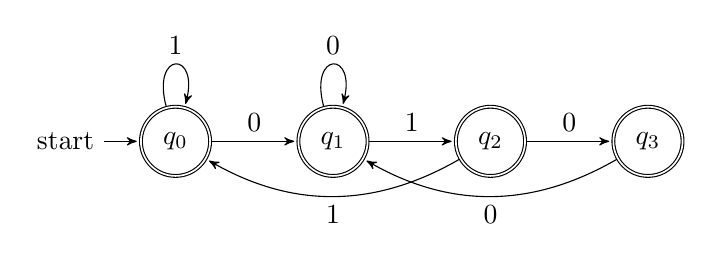
\begin{tikzpicture}[>=stealth',shorten >=1pt,auto,node distance=2cm]
                \node[initial,state,accepting] (q0)      {$q_0$};
                \node[state,accepting] (q1) [right of=q0]     {$q_1$};
                \node[state,accepting] (q2) [right of=q1]     {$q_2$};
                \node[state,accepting] (q3) [right of=q2]     {$q_3$};                               
                \path[->]
                    (q0) edge[loop above] node {$1$} (q0)
                    (q0) edge node {$0$} (q1)
                    (q1) edge[loop above] node {$0$} (q1)
                    (q1) edge node {$1$} (q2)
                    (q2) edge node {$0$} (q3)
                    (q2) edge[bend left] node {$1$} (q0)
                    (q3) edge[bend left] node {$0$} (q1)
                ;
            \end{tikzpicture}
        \end{center}
        
    \end{itemize}
    Construct a pushdown automaton recognizing the intersection $L=L_1\cap L_2$ of the lanugages $L_1$ and $L_2$.

\end{problem}


\end{document}
